\section{Analyse der Anforderungen}
\subsection{Rollen im IT-System}
Anhand der Stakeholderanalyse und der Spezifikation der funktionalen Anforderungen wurden mehrere Akteure ermittelt, die mit dem System interagieren und später im Programm als Benutzerrolle umgesetzt werden sollen:
\begin{itemize}
    \item[] \underline{Administrator:} Die Rolle des Administrator ist in den Anforderungen \emph{/F21/} bis \emph{/F23/} beschrieben und ist für die Verwaltung des Systems zuständig, indem er Benutzer anlegt, ihnen Rollen zuweist und Projekte erstellt. Er kann außerdem alle Projekte und darin enthaltenen Teilprojekte einsehen und Änderungen vornehmen. Verkörpert werden die Administratoren durch die Mitarbeiter des oberen Managements des auftraggebenen Unternehmen.
    
    \item[] \underline{Projektleiter:} Die Rolle des Projektleiter ist in den Anforderungen \emph{/F24/} bis \emph{/F26/} beschrieben und kann ist für die Erstellung und Administration seiner Projekte im System veranwortlich. Im Gegensatz zum Administrator hat der Projektleiter keine vollständigen, globalen Berechtigungen sondern diese nur in seinem eigenen Projekt und kann dort z.B. Teilprojekte anlegen, Projektphasen definieren und Mitarbeiter zuordnen. Zum Ende einer Projektphase kann der Projektleiter die Phase für die Bearbeitung sperren. Auf fremde Projekte hat der Projektleiter keinen Zugriff. 
    
    \item[] \underline{Teilprojektleiter:} Die Rolle des Teilprojektleiter ist in der Anforderung \emph{/F27/} beschrieben und ist für die Verwaltung des ihm zugeordneten Teilprojekts zuständig. In diesem kann er sämtliche Aktionen durchführen, wie z.B. das Bearbeiten von Projektphasenattributen, das Anlegen von Prozessen, Subprozessen und Prozessschritten und das Erfassen des aktuellen Fortschrittes. Des Weiteren haben Teilprojektleiter Lesezugriff auf fremde Teilprojekte im selben Projekt, um beispielweise Informationen zu übergreifenden Prozessen zu erlangen.

    \item[] \underline{Projektmitarbeiter:} Die Rolle des Projektmitarbeiters ist in der Anforderung \emph{/F28/} beschrieben und ist für die Erfassung in den jeweiligen Teilprojekten zuständig. Der Projektmitarbeiter ist einem Teilprojekt zugeordnet und kann dort Prozesse, Subprozesse und Prozessschritte anlegen und den aktuellen Status erfassen, indem die Attribute der aktuellen Projektphase entsprechend ausgeprägt werden.

    \item[] \underline{Kunde:} Die Rolle des Kunden ist in der Anforderung \emph{/F26/} beschrieben und soll den Kunden, in deren Kontext das jeweilige Projekt stattfindet, Zugriff auf das System gewähren. Die Kunden erhalten dabei standardmäßig jeweils nur Lesezugriff auf ihr eigenes Projekt, damit die Fortschritte im Projekt nachvollzogen werden können. Es besteht die Möglichkeit den Benutzern Schreibrechte zu erteilen, entweder für das ganze Projekt, oder nur für einzelne Teilprojekte, um den Fall zu ermöglichen, das Mitarbeiter des Kunden ebenfalls mit dem BTT arbeiten.  

\end{itemize}

\subsection{Anwendungsfälle}
Nachfolgend werden die funktionalen Anforderungen durch Anwendungsfälle genauer erklärt. Für die Beschreibung wird auf eine Anwendungsfallschablone zurückgegriffen, die die Eigenschaften des Anwendungsfall systematisch abfragt. Die Eigenschaften sind, das Ziel des Anwendungsfall, die Kategorie, die angibt wie häufig der Anwendungsfall ausgeführt wird, die Vorbedingung, die Nachbedingung bei Erfolg, die Nachbedingung bei Misserfolg, die Akteure des Anwendungsfall, das Auslösende Ereignis, die Beschreibung in einzelnen Schritten, die Erweiterung und mögliche Alternativen.\footcite[Vgl.][S. 261]{balzert}
\begin{figure}[h]
    \centering
    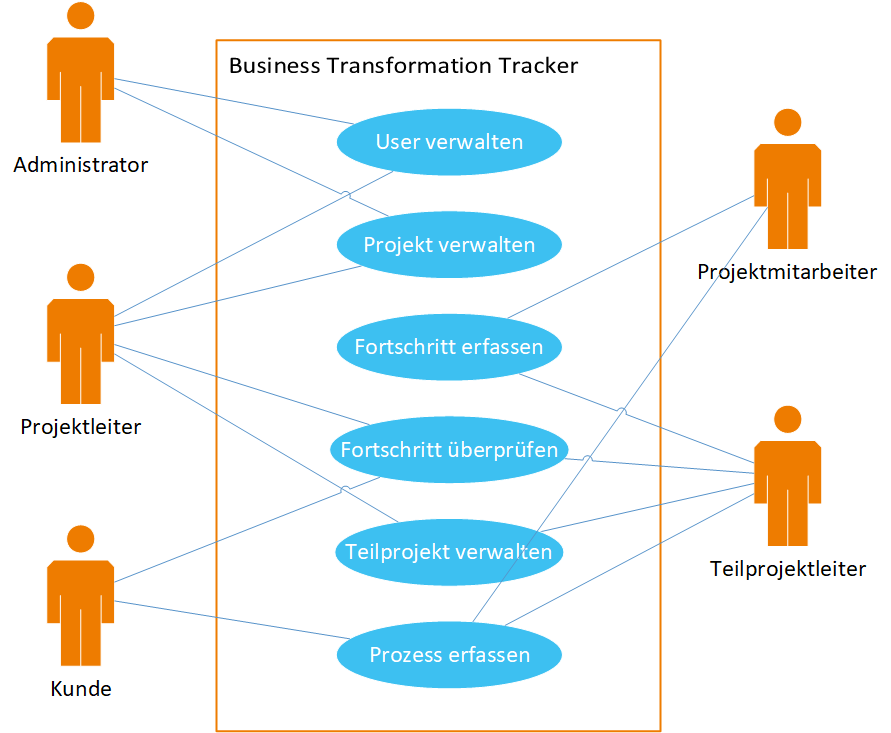
\includegraphics[scale=0.67]{./Bilder/Anwendungsfalldiagramm.png}
    \caption[Anwendungsfalldiagramm]{Anwendungsfalldiagramm mit Akteueren}
    \label{fig:Anwendungsfalldiagramm}
\end{figure}
In Abbildung \ref{fig:Anwendungsfalldiagramm} ist eine Übersicht der aus den Anforderungen erarbeiteten Anwendungsfälle zu sehen, die in den nachfolgenden Unterkapiteln anhand der oben beschriebenen Schablone genauer beschrieben werden.

\subsubsection{Anwendungsfall 1: User verwalten}
\underline{\emph{Ziel:}}\\
Es werden die für einen User hinterlegten Daten geändert. Dies kann zum einen das Passwort sein, aber auch die Stammdaten, die Rolle, oder die Zuordnung zu einem Projekt, oder Teilprojekt.\\
\underline{\emph{Kategorie:}} \\
Sekundär\\
\underline{\emph{Vorbedingung:}} \\
Der Anwender hat sich zuvor im System mit seinem Benutzernamen und Passwort angemeldet.\\
\underline{\emph{Nachbedingung Erfolg:}} \\
Die Daten und Zuordnungen des Benutzer wurden wie gewünscht angepasst.\\
\underline{\emph{Nachbedingung Fehlschlag:}} \\
Die Daten und Zuordnungen des Benutzers bleiben unverändert.\\
\underline{\emph{Akteure:}} \\
Administrator, Projektleiter\\
\underline{\emph{Auslösendes Ereignis:}} \\
Die Daten oder Zuordnungen des Benutzer müssen angepasst werden.\\
\underline{\emph{Beschreibung:}}
\begin{itemize}
    \item [1] Die Benutzerübersicht wird aufgerufen
    \item [2] Der gewünschte Benutzer wird ausgewählt.
    \item [3] Die Stammdaten des Benutzer werden editiert.
    \item [4] Die veränderten Daten werden gesichert.
\end{itemize}
\underline{\emph{Erweiterung:}}
\begin{itemize}
    \item [2a] Der Nutzer ist nicht vorhanden und wird angelegt.
    \item [3a] Der Benutzer wird einem Projekt zugeordnet.
    \item [3b] Der Benutzer wird einem Teilprojekt zugeordnet.
    \item [3c] Der Benutzer wird aus einem Projekt gelöscht.
    \item [3d] Der Benutzer wird aus einem Teilprojekt gelöscht.
    \item [3e] Das Passwort des Benutzer wird zurückgesetzt.
\end{itemize}
\underline{\emph{Alternativen:}}
\begin{itemize}
    \item [2b] Der Benutzer wird gelöscht.
    \item [3f] Die Daten sind korrekt und der Vorgang wird abgebrochen.
\end{itemize}

\subsubsection{Anwendungsfall 2: Projekt anlegen}
\underline{\emph{Ziel:}}\\
Ein neues Projekt wird hinzugefügt und die Stammdaten des Projekts werden erfasst.\\
\underline{\emph{Kategorie:}} \\
Primär\\
\underline{\emph{Vorbedingung:}} \\
Der Anwender hat sich zuvor im System mit seinem Benutzernamen und Passwort angemeldet und das Projekt ist noch nicht angelegt.\\
\underline{\emph{Nachbedingung Erfolg:}} \\
Das Projekt wird angelegt und die Stammdaten des Projekts werden wie gewünscht hinterlegt, die benötigten Projektphasen sind vorhanden und Teilprojekte sind ebenfalls angelegt.\\
\underline{\emph{Nachbedingung Fehlschlag:}} \\
Es wird kein Projekt angelegt.\\
\underline{\emph{Akteure:}} \\
Administrator, Projektleiter\\
\underline{\emph{Auslösendes Ereignis:}} \\
Es wird ein neues Projekt begonnen.\\
\underline{\emph{Beschreibung:}}
\begin{itemize}
    \item [1] Der Anwender ruft die Projektübersicht auf.
    \item [2] Ein neues Projekt wird hinzugefügt.
    \item [3] Die Stammdaten des Projekts werden hinterlegt, in Form eines Bezeichners, Beschreibung, Projektzeitraum, Kunde, und ggf. Bemerkungen.
    \item [4] Es wird ein Teilprojekt hinzugefügt.
    \item [5] Es wird eine Projektphase hinzugefügt.
    \item [6] Es werden die vorgesehenen Mitarbeiter hinzugefügt.
    \item [7] Die veränderten Daten werden gesichert.
\end{itemize}
\underline{\emph{Erweiterung:}} \\
\begin{itemize}
    \item [4a] Es werden weitere Teilprojekte hinzugefügt. 
    \item [5a] Es werden weitere Projektphasen hinzugefügt.
    \item [5b] Die Attribute der Projektphasen, die standardmäßig vorgegeben sind, werden angepasst. 
\end{itemize}
\underline{\emph{Alternativen:}} \\
\begin{itemize}
    \item  
\end{itemize}

\subsubsection{Anwendungsfall 3: Fortschritt erfassen}
\underline{\emph{Ziel:}}\\
\\
\underline{\emph{Kategorie:}} \\
Primär\\
\underline{\emph{Vorbedingung:}} \\
Der Anwender hat sich zuvor im System mit seinem Benutzernamen und Passwort angemeldet.\\
\underline{\emph{Nachbedingung Erfolg:}} \\
\\
\underline{\emph{Nachbedingung Fehlschlag:}} \\
\\
\underline{\emph{Akteure:}} \\
Teilprojektleiter, Projektmitarbeiter\\
\underline{\emph{Auslösendes Ereignis:}} \\
\\
\underline{\emph{Beschreibung:}} \\
\\
\underline{\emph{Erweiterung:}} \\
\\
\underline{\emph{Alternativen:}} \\
\\

\subsubsection{Anwendungsfall 4: Fortschritt überprüfen}
\underline{\emph{Ziel:}}\\
\\
\underline{\emph{Kategorie:}} \\
Sekundär\\
\underline{\emph{Vorbedingung:}} \\
Der Anwender hat sich zuvor im System mit seinem Benutzernamen und Passwort angemeldet.\\
\underline{\emph{Nachbedingung Erfolg:}} \\
\\
\underline{\emph{Nachbedingung Fehlschlag:}} \\
\\
\underline{\emph{Akteure:}} \\
Projektleiter, Teilprojektleiter, Kunde\\
\underline{\emph{Auslösendes Ereignis:}} \\
\\
\underline{\emph{Beschreibung:}} \\
\\
\underline{\emph{Erweiterung:}} \\
\\
\underline{\emph{Alternativen:}} \\
\\

\subsubsection{Anwendungsfall 5: Teilprojekt verwalten}
\underline{\emph{Ziel:}}\\
\\
\underline{\emph{Kategorie:}} \\
Sekundär\\
\underline{\emph{Vorbedingung:}} \\
Der Anwender hat sich zuvor im System mit seinem Benutzernamen und Passwort angemeldet.\\
\underline{\emph{Nachbedingung Erfolg:}} \\
\\
\underline{\emph{Nachbedingung Fehlschlag:}} \\
\\
\underline{\emph{Akteure:}} \\
Projektleiter, Teilprojektleiter\\
\underline{\emph{Auslösendes Ereignis:}} \\
\\
\underline{\emph{Beschreibung:}} \\
\\
\underline{\emph{Erweiterung:}} \\
\\
\underline{\emph{Alternativen:}} \\
\\

\subsubsection{Anwendungsfall 6 Prozess erfassen}
\underline{\emph{Ziel:}}\\
\\
\underline{\emph{Kategorie:}} \\
Primär\\
\underline{\emph{Vorbedingung:}} \\
Der Anwender hat sich zuvor im System mit seinem Benutzernamen und Passwort angemeldet.\\
\underline{\emph{Nachbedingung Erfolg:}} \\
\\
\underline{\emph{Nachbedingung Fehlschlag:}} \\
\\
\underline{\emph{Akteure:}} \\
Teilprojektleiter, Projektmitarbeiter, Kunde\\
\underline{\emph{Auslösendes Ereignis:}} \\
\\
\underline{\emph{Beschreibung:}} \\
\\
\underline{\emph{Erweiterung:}} \\
\\
\underline{\emph{Alternativen:}} \\
\\



\subsection{Benutzerollen und Berechtigungen}
\subsection{Use-Cases}
\subsection{Sequenzdiagramme}


\begin{comment}
        
%überarbeiten, an neues Buch anpassen
%Anforderungen --> Anforderungsspezifikation --> Fachliche Lösung
In dem nun folgendem Kapitel wird die Anforderungsanalyse behandelt. Orientiert wird sich dazu an dem Vorgehensmodell von Helmut Balzert, das ausführlich in dem Modul BIS-134 Anforderungsanalyse des Studiengangs Wirtschaftsinformatik der Hochschule Hannover behandelt wurde.\\Die Anforderungsanalyse ist einer der ersten Schritte im Softwareentwicklungsprozess und hat zum Ziel die Anforderungen zu ermitteln, die das System, in diesem Fall der Business Transformation Tracker, leisten soll, sowie diese zu definieren. Dadurch soll eine größtmögliche Abdeckung der gestellten Anforderungen erreicht werden und Unstimmigkeiten mit dem Kunden, bzw. dem Auftraggeber, in Bezug auf Funktion und Umfang, vermieden werden. Im Wasserfallmodell nach Balzert ist die Anforderungsanalyse in der Definitionsphase verortert und arbeitet somit mit den Ergebnisobjekten der vorangegangenen Planungsphase. \footcite[Vgl.][S. 100 ff.]{balzert} Die Ergebnisse der Anforderungsanalyse werden dem anschließenden Kapitel, der Konzeption und somit der Entwurfsphase, als Basis dienen.\\
Im Rahmen dieser    Darstellung in UML


\subsection{Ermittlung der Anforderungen}
Im nachfolgendem Kapitel werden die Anforderungen an die Software, die sich aus der Problemstellung und Gesprächen mit dem Auftraggeber ergeben haben, genauer spezifiziert. Im Anschluss folgen dann die zusätzlichen Anforderungen, die sich aus der Umfrage ergeben haben.

\subsubsection{Nichtfunktionale Anforderungen}
%Anforderungen müssen systematisch gewonnen werden von Beteiligten und Betroffenen, sonstige quellen

\subsection{Spezifizierung der Anforderungen}
%Ermittelte Anforderungen müssen spezifiziert werden, unter Berücksichtigung von festgelegten Methoden, Richtlinien, etc.

\subsection{Analyse der Anforderungen}
%Spezifizierte Anforderungen müssen anhand von Richtlinien und Checklisten analysiert werden

\subsection{Modellierung der Anforderungen}
%analysierte und validierte Anforderungen bilden Ausgangspunkt für Modellierung der fachlichen Lösung

\subsection{Verifikation der Anforderungen}

\subsection{Wahl der Entwicklungsplattform}
warum java, nicht web, nicht abap, nicht etc..
bewertung der it sicherheit anhand bestimmter kriterien (datenschutz, zugriffssicherheit, bewahrung von geschäftsgeheimnissne), java weil protierung auf allen plattformen (windows, unix, macos) verfügbar

\subsection{Pflichtenheft}
Durch den Auftraggeber wurden folgende Anforderungen gestellt:

\subsection{Use-Cases}
Akteure des IT-Systems definieren
Mitarbeiter: Projektmitarbeiter, Projektleiter, Teilprojektleiter
Usecase 1:
Der Projektleiter möchte ein neues Projekt anlegen und die Mitarbeiter zuordnen

Usecase 2:
Der Teilprojektleiter öffnet ein vorhandenes Projekt und fügt erfasst die Prozesse und Subprozesse

Usecase 3:
Ein Projektmitarbeiter möchte den aktuellen Fortschritt in einem Subprozess erfassen.

\subsection{Umgebung}
\subsection{Schnittstellen}

%Methodik
\begin{comment}
    %Methodik
    --> Wasserfallmodell nach Helmut Balzert(1995), S.100 ff.

    Anwendungsfälle
    Geschäftsprozessdiagramm, Aktivitätsdiagramm (Folie 94)
    Anwendungsfalldiagramm, -schablone
    Klassendiagramme --> Beziehungen --> Detailliertes Klassendiagramme
    Attribute Spezifizieren (exemplarisch), Operationen
    Sequenzdiagramm

    Pflichtenheft (genaue spezifizierung) 
    Verfeinerung des Lastenheftes
    Verbale Beschreibung dessen, was das System leisten soll (Auftraggebersicht)
    Dient i. a. als vertragliche Beschreibung des Lieferumfangs
    Einstiegsdokument für alle, die das System später pflegen und warten sollen
    Grundlage für die Erstellung des Produkt-Modells

    Ziel
    •Präzise Festlegung, WAS das System leisten soll (aus Sicht des Auftraggebers)
    Anforderungsanalyse
    •Ermittlung und Beschreibung der Anforderungen des Auftraggebers an ein IT-System
    •Bestimmung dessen, WAS das System leisten soll
    •Erstellen eines logischen Modells

\end{comment}